\section{Results}
\label{sec:results}
    \begin{figure*}
      \centering
      \subfigure[Linguistics]{
        \begin{tikzpicture}[scale=.5925]
          \pgfkeys{/pgf/number format/.cd, fixed}
          \begin{axis}[x=0.0076038\linewidth,
                       xtick={0, 20, 40, ..., 100},
                       xmin=0,
                       xmax=40,
                       xlabel=recall (\%),
                       x label style={yshift=.34em},
                       y=0.0076038\linewidth,
                       ytick={0, 10, 20, ..., 100},
                       ymin=0,
                       ymax=40,
                       ylabel=precision (\%),
                       y label style={yshift=-1.1em},
                       legend style={font=\footnotesize}]
            \addplot [red, mark=+] file {input/data/linguistique_topicrank.csv};
            \addplot [green, mark=o] file {input/data/linguistique_kea_pp.csv};
            \addplot [blue, mark=x] file {input/data/linguistique_topiccorank.csv};
            \addplot [dotted, domain=20:40] {(30 * x) / ((2 * x) - 30)};
            \addplot [dotted, domain=10:40] {(20 * x) / ((2 * x) - 20)};
            \addplot [dotted, domain=5:40] {(10 * x) / ((2 * x) - 10)};
            %\legend{TopicRank, KEA++, TopicCoRank};
          \end{axis}
          \node at (4.9,3.1) [anchor=east] {\scriptsize{F=30.0}};
          \node at (4.9,1.8) [anchor=east] {\scriptsize{F=20.0}};
          \node at (4.9,0.9) [anchor=east] {\scriptsize{F=10.0}};
        \end{tikzpicture}
      }
      \subfigure[Archaeology]{
        \begin{tikzpicture}[scale=.5925]
          \pgfkeys{/pgf/number format/.cd, fixed}
          \begin{axis}[x=0.0050692\linewidth,
                       xtick={0, 20, 40, ..., 100},
                       xmin=0,
                       xmax=60,
                       xlabel=recall (\%),
                       x label style={yshift=.34em},
                       y=0.0050692\linewidth,
                       ytick={0, 15, 30, ..., 100},
                       ymin=0,
                       ymax=60,
                       ylabel=precision (\%),
                       y label style={yshift=-1.1em},
                       legend style={font=\footnotesize}]
            \addplot [red, mark=+] file {input/data/archeologie_topicrank.csv};
            \addplot [green, mark=o] file {input/data/archeologie_kea_pp.csv};
            \addplot [blue, mark=x] file {input/data/archeologie_topiccorank.csv};
            \addplot [dotted, domain=30:60] {(40 * x) / ((2 * x) - 40)};
            \addplot [dotted, domain=20:60] {(30 * x) / ((2 * x) - 30)};
            \addplot [dotted, domain=10:60] {(20 * x) / ((2 * x) - 20)};
            \addplot [dotted, domain=5:60] {(10 * x) / ((2 * x) - 10)};
            %\legend{TopicRank, KEA++, TopicCoRank};
          \end{axis}
          \node at (4.9,2.65) [anchor=east] {\scriptsize{F=40.0}};
          \node at (4.9,1.85) [anchor=east] {\scriptsize{F=30.0}};
          \node at (4.9,1.15) [anchor=east] {\scriptsize{F=20.0}};
          \node at (4.9,0.65) [anchor=east] {\scriptsize{F=10.0}};
        \end{tikzpicture}
      }
      \subfigure[DUC]{
        \begin{tikzpicture}[scale=.5925]
          \pgfkeys{/pgf/number format/.cd, fixed}
          \begin{axis}[x=0.0050692\linewidth,
                       xtick={0, 20, 40, ..., 100},
                       xmin=0,
                       xmax=60,
                       xlabel=recall (\%),
                       x label style={yshift=.34em},
                       y=0.0050692\linewidth,
                       ytick={0, 15, 30, ..., 100},
                       ymin=0,
                       ymax=60,
                       ylabel=precision (\%),
                       y label style={yshift=-1.1em},
                       legend style={font=\footnotesize}]
            \addplot [red, mark=+] file {input/data/duc_topicrank.csv};
            \addplot [blue, mark=x] file {input/data/duc_topiccorank.csv};
            \addplot [dotted, domain=30:60] {(40 * x) / ((2 * x) - 40)};
            \addplot [dotted, domain=20:60] {(30 * x) / ((2 * x) - 30)};
            \addplot [dotted, domain=10:60] {(20 * x) / ((2 * x) - 20)};
            \addplot [dotted, domain=5:60] {(10 * x) / ((2 * x) - 10)};
            %\legend{TopicRank, TopicCoRank};
          \end{axis}
          \node at (4.9,2.65) [anchor=east] {\scriptsize{F=40.0}};
          \node at (4.9,1.85) [anchor=east] {\scriptsize{F=30.0}};
          \node at (4.9,1.15) [anchor=east] {\scriptsize{F=20.0}};
          \node at (4.9,0.65) [anchor=east] {\scriptsize{F=10.0}};
        \end{tikzpicture}
      }
      \subfigure[SemEval]{
        \begin{tikzpicture}[scale=.5925]
          \pgfkeys{/pgf/number format/.cd, fixed}
          \begin{axis}[x=0.0076038\linewidth,
                       xtick={0, 20, 40, ..., 100},
                       xmin=0,
                       xmax=40,
                       xlabel=recall (\%),
                       x label style={yshift=.34em},
                       y=0.0076038\linewidth,
                       ytick={0, 10, 20, ..., 100},
                       ymin=0,
                       ymax=40,
                       ylabel=precision (\%),
                       y label style={yshift=-1.1em},
                       legend style={font=\Large}]
            \addplot [red, mark=+] file {input/data/semeval_topicrank.csv};
            \addplot [green, mark=o] coordinates {
                (-1.0, -1.0)
            };
            \addplot [blue, mark=x] file {input/data/semeval_topiccorank.csv};
            \addplot [dotted, domain=20:40] {(30 * x) / ((2 * x) - 30)};
            \addplot [dotted, domain=10:40] {(20 * x) / ((2 * x) - 20)};
            \addplot [dotted, domain=5:40] {(10 * x) / ((2 * x) - 10)};
            \legend{TopicRank, KEA++, TopicCoRank};
          \end{axis}
          %\node at (4.9,3.1) [anchor=east] {\scriptsize{F=30.0}};
          \node at (4.9,1.8) [anchor=east] {\scriptsize{F=20.0}};
          \node at (4.9,0.9) [anchor=east] {\scriptsize{F=10.0}};
        \end{tikzpicture}
      }
      \caption{Precision-recall curves of TopicRank, KEA++ and TopicCoRank
               for each dataset
               \label{fig:pr_curves1}}
    \end{figure*}
    
    \begin{figure*}
      \centering
      \subfigure[Linguistics]{
        \begin{tikzpicture}[scale=.525]
          \pgfkeys{/pgf/number format/.cd, fixed}
          \begin{axis}[x=0.00349508\linewidth,
                       xtick={0, 20, ..., 100},
                       xmin=0.0,
                       xmax=100.0,
                       xlabel=Assignment ratio (\%),
                       x label style={yshift=.34em},
                       y=0.016675\textheight,
                       ytick={0, 2, 4, ..., 34},
                       ymin=14,
                       ymax=28,
                       ylabel=f-score (\%),
                       y label style={yshift=-1.1em}]
            \addplot[blue, mark=x] coordinates{
              (0, 15.42)
              (10, 16.56)
              (20, 17.23)
              (30, 17.73)
              (40, 18.54)
              (50, 19.56)
              (60, 20.78)
              (70, 22.31)
              (80, 23.85)
              (90, 25.29)
              (100, 26.18)
            };
          \end{axis}
        \end{tikzpicture}
      }
      \subfigure[Archaeology]{
        \begin{tikzpicture}[scale=.525]
          \pgfkeys{/pgf/number format/.cd, fixed}
          \begin{axis}[x=0.00349508\linewidth,
                       xtick={0, 20, ..., 100},
                       xmin=0.0,
                       xmax=100.0,
                       xlabel=Assignment ratio (\%),
                       x label style={yshift=.34em},
                       y=0.016675\textheight,
                       ytick={0, 2, 4, ..., 42},
                       ymin=28,
                       ymax=42,
                       ylabel=f-score (\%),
                       y label style={yshift=-1.1em}]
            \addplot[blue, mark=x] coordinates{
              (0, 28.69)
              (10, 28.77)
              (20, 29.09)
              (30, 29.29)
              (40, 29.65)
              (50, 30.43)
              (60, 31.46)
              (70, 33.31)
              (80, 34.83)
              (90, 36.40)
              (100, 38.50)
            };
          \end{axis}
        \end{tikzpicture}
      }
      \subfigure[DUC]{
        \begin{tikzpicture}[scale=.525]
          \pgfkeys{/pgf/number format/.cd, fixed}
          \begin{axis}[x=0.00349508\linewidth,
                       xtick={0, 20, ..., 100},
                       xmin=0.0,
                       xmax=100.0,
                       xlabel=Assignment ratio (\%),
                       x label style={yshift=.34em},
                       y=0.016675\textheight,
                       ytick={0, 2, 4, ..., 38},
                       ymin=24,
                       ymax=38,
                       ylabel=f-score (\%),
                       y label style={yshift=-1.1em}]
            \addplot[blue, mark=x] coordinates{
              (0, 28.15)
              (10, 29.97)
              (20, 30.95)
              (30, 32.15)
              (40, 33.00)
              (50, 32.86)
              (60, 32.34)
              (70, 31.59)
              (80, 30.99)
              (90, 30.29)
              (100, 29.44)
            };
          \end{axis}
        \end{tikzpicture}
      }
      \subfigure[SemEval]{
        \begin{tikzpicture}[scale=.525]
          \pgfkeys{/pgf/number format/.cd, fixed}
          \begin{axis}[x=0.00349508\linewidth,
                       xtick={0, 20, ..., 100},
                       xmin=0.0,
                       xmax=100.0,
                       xlabel=Assignment ratio (\%,
                       x label style={yshift=.34em},
                       y=0.016675\textheight,
                       ytick={0, 2, 4, ..., 34},
                       ymin=8,
                       ymax=22,
                       ylabel=f-score (\%),
                       y label style={yshift=-1.1em}]
            \addplot[blue, mark=x] coordinates{
              (0, 12.36)
              (10, 13.04)
              (20, 13.72)
              (30, 13.56)
              (40, 13.43)
              (50, 12.79)
              (60, 12.68)
              (70, 11.50)
              (80, 11.06)
              (90, 10.78)
              (100, 9.69)
            };
          \end{axis}
        \end{tikzpicture}
      }
      \caption{Behavior of TopicCoRank's f-score (F) regarding the assignment ratio
               for each dataset
               \label{fig:assignment_ratio_variations}}
    \end{figure*}
    
    Table~\ref{tab:comparison_results} shows the results obtained with
    TopicCoRank and the baselines for each of the datasets. Overall, we observe that TopicCoRank significantly outperforms TopicRank and KEA++. Surprisingly, KEA++  achieves low performance. The main reason is that a large proportion of the controlled keyphrases do not occur within the documents ($\simeq$50\%). We also observed that the thesauri we use, which are real case scenario thesauri, contain less semantic relations than the one applied by \newcite{medelyan2006kea++} on random documents from the UN Food and Agriculture Organization (FAO). Concerning TopicCoRank and its variants, TopicCoRank performs better on DUC and SemEval, while its assignment variant, TopicCoRank$_\textnormal{\textit{assign}}$, performs better on Linguistics and Archaeology. The annotation strategy of the professional indexers is centered on controlled vocabularies, which explains why the assignment should be prioritized on the case of Linguistics and Archaeology. However, by better performing, TopicCoRank$_\textnormal{\textit{assign}}$ shows that the ranking of the controlled keyphrases efficiently gives importance to the controlled keyphrases in the context of the document. Therefore, connecting document topics to controlled keyphrases is useful for the ranking.

    Moreover, the results we observe on DUC are highly competitive with the best reported
    results on DUC (31.7\% of f-score)~\cite{wan2008expandrank} and higher than the best
    reproduced results (26.4\% of f-score)~\cite{hassan2010conundrums}.
  
    Precision-recall curves displayed in figure~\ref{fig:pr_curves1}, confirms the
    previous observations. In term of optimizing precision and recall, TopicCoRank
    dominates both TopicRank and KEA++, which means that TopicCoRank achieves the
    best performance for any precision and recall values.
  
    Table~\ref{tab:assignment_ratio} shows the percentage of keyphrases assigned by
    TopicCoRank at 10 keyphrases for each dataset. As we claimed, the percentage of assigned keyphrases per document shows that TopicCoRank independently assigns and extracts keyphrases. 
    \begin{table}[!h]
        \centering
        \begin{tabular}{l|c}
            \toprule
            & Assignment ratio\\
            \hline
            Linguistics & 38.7\%\\
            Archaeology & 32.2\%\\
            DUC & 58.6\%\\
            SemEval & 40.0\%\\
            \bottomrule
        \end{tabular}
        \caption{Average ratio of assignment performed by TopicCoRank at 10 keyphrases
                 \label{tab:assignment_ratio}}
    \end{table}
    
    \begin{figure*}
      \centering
      \subfigure[Linguistics]{
        \begin{tikzpicture}[scale=.7425]
          \pgfkeys{/pgf/number format/.cd, fixed}
          \begin{axis}[x=0.262\linewidth,
                       xtick={0.1, 0.3, ..., 0.9},
                       xmin=0.05,
                       xmax=0.95,
                       xlabel=$\lambda$,
                       x label style={yshift=.34em},
                       y=0.0125\textheight,
                       ytick={0, 2, 4, ..., 34},
                       ymin=14,
                       ymax=26,
                       ylabel=f-score (\%),
                       y label style={yshift=-1.1em}]
            \addplot[blue, mark=x] coordinates{
              (0.1, 20.04)
              (0.2, 20.22)
              (0.3, 20.37)
              (0.4, 20.14)
              (0.5, 20.09)
              (0.6, 18.46)
              (0.7, 16.69)
              (0.8, 15.98)
              (0.9, 16.43)
            };
          \end{axis}
        \end{tikzpicture}
      }
      \subfigure[Archaeology]{
        \begin{tikzpicture}[scale=.7425]
          \pgfkeys{/pgf/number format/.cd, fixed}
          \begin{axis}[x=0.262\linewidth,
                       xtick={0.1, 0.3, ..., 0.9},
                       xmin=0.05,
                       xmax=0.95,
                       xlabel=$\lambda$,
                       x label style={yshift=.34em},
                       y=0.0125\textheight,
                       ytick={0, 2, 4, ..., 36},
                       ymin=24,
                       ymax=36,
                       ylabel=f-score (\%),
                       y label style={yshift=-1.1em}]
            \addplot[blue, mark=x] coordinates{
              (0.1, 32.20)
              (0.2, 31.74)
              (0.3, 31.58)
              (0.4, 31.33)
              (0.5, 31.09)
              (0.6, 30.64)
              (0.7, 28.96)
              (0.8, 26.52)
              (0.9, 24.61)
            };
          \end{axis}
        \end{tikzpicture}
      }
      \subfigure[DUC]{
        \begin{tikzpicture}[scale=.7425]
          \pgfkeys{/pgf/number format/.cd, fixed}
          \begin{axis}[x=0.262\linewidth,
                       xtick={0.1, 0.3, ..., 0.9},
                       xmin=0.05,
                       xmax=0.95,
                       xlabel=$\lambda$,
                       x label style={yshift=.34em},
                       y=0.0125\textheight,
                       ytick={0, 2, 4, ..., 36},
                       ymin=24,
                       ymax=36,
                       ylabel=f-score (\%),
                       y label style={yshift=-1.1em}]
            \addplot[blue, mark=x] coordinates{
              (0.10, 31.96)
              (0.20, 32.24)
              (0.30, 32.40)
              (0.40, 31.92)
              (0.50, 31.53)
              (0.60, 30.50)
              (0.70, 28.23)
              (0.80, 26.61)
              (0.90, 24.63)
            };
          \end{axis}
        \end{tikzpicture}
      }
      \subfigure[SemEval]{
        \begin{tikzpicture}[scale=.7425]
          \pgfkeys{/pgf/number format/.cd, fixed}
          \begin{axis}[x=0.262\linewidth,
                       xtick={0.1, 0.3, ..., 0.9},
                       xmin=0.05,
                       xmax=0.95,
                       xlabel=$\lambda$,
                       x label style={yshift=.34em},
                       y=0.0125\textheight,
                       ytick={0, 2, 4, ..., 34},
                       ymin=8,
                       ymax=20,
                       ylabel=f-score (\%),
                       y label style={yshift=-1.1em}]
            \addplot[blue, mark=x] coordinates{
              (0.10, 11.24)
              (0.20, 11.33)
              (0.30, 11.39)
              (0.40, 12.07)
              (0.50, 13.43)
              (0.60, 14.49)
              (0.70, 14.09)
              (0.80, 13.96)
              (0.90, 13.28)
            };
          \end{axis}
        \end{tikzpicture}
      }
      \caption{Behavior of TopicCoRank's f-score (F) regarding the value of $\lambda$
               for each dataset
               \label{fig:lambda_variations}}
    \end{figure*}

    Furthermore, we artificially vary the assignment ratio and show the resulting performances of TopicCoRank in figure~\ref{fig:assignment_ratio_variations}. Results also show the difference between the two Linguistics and Archaeology datasets and the two DUC and SemEval datasets. On Linguistics and Archaeology, the performance of TopicCoRank is in the form of a pseudo-cumulative curve: the more TopicCoRank assigns, the better it performs. On DUC and SemEval, the performance of TopicCoRank is in the form of a pseudo-normal curve: extraction and assignment must be balanced to achieve better results.
    Linguistics and Archaeology have been annotated with a strong focus on controlled vocabulary, which explains why assignment should be prioritized. DUC and SemEval have been freely annotated. In that case, the default TopicCoRank, which tends to balance assignment and extraction, achieves a near optimal performance.
    
    Additionally, figure~\ref{fig:lambda_variations} shows the behavior of TopicCoRank
    regarding the value of $\lambda$, which configures the importance of the inner
    recommendation over the outer recommendation. Globally, we can see that balancing
    the recommendation between the inner and the outer recommendation induces
    near-optimal performances. This observation indicates that the specific domain of a
    document is as important as the content of the document.
    
    Finally, we provide insights of the improvement of TopicCoRank over TopicRank with
    an example of keyphrase annotation for the document \texttt{FT941-1547} of DUC, namely
    \textit{Commodities and Agriculture: Germany sets scientist to work}, which talks about
    a German research project to examine whether the cattle disease bovine spongiform
    encephalopathy (BSE) can be transmitted to human beings:
    \begin{center}
        \begin{varwidth}{.9\linewidth}
            \textbf{Reference}:
            \begin{enumerate*}
                \item{cattle disease;}
                \item{bovine spongiform encephalopathy;}
                \item{BSE;}
                \item{mad cow disease;}
                \item{British beef imports;}
                \item{possible connections.}
            \end{enumerate*}
            \noindent\rule[0.5ex]{\linewidth}{.5pt}
            \textbf{TopicRank}:
            \begin{enumerate*}
                \item{\underline{British beef imports};}
                \item{human beings;}
                \item{new research project;}
                \item{disease;}
                \item{non-existent;}
                \item{German universities.}
            \end{enumerate*}\\
            \textbf{TopicCoRank}:
            \begin{enumerate*}
                \item{\underline{British beef imports};}
                \item{\underline{BSE};}
                \item{\underline{mad cow disease};}
                \item{ban;}
                \item{\underline{bovine spongiform encephalopathy};}
                \item{Germany.}
            \end{enumerate*}
        \end{varwidth}
    \end{center}
    Underlined keyphrases correspond to correctly extracted and assigned keyphrases.
